\section{The Nuclear Fuel Cycle}
\label{sec:nfc}

The \acrlong{nfc} (NFC) is comprised of a series of industrial processes that
produce and consume nuclear fuel, here we present a high-level overview to
establish the context for our work with modeling the fuel cycle in later chapters. Commonly, these processes are grouped into two categories (the front
end and back end). In the \gls{usa}, we keep each of these facilities separate
in the front end of the fuel cycle in a "collect and wait" pathway
\cite{cycle_risks}. Without a long-term or interim solution for the \gls{uf},
the back end of the \gls{nfc} is collocated with the reactors that burn the
fuel (with the minor exception of the consolidated storage facility in Morris
Illinois). For this work, we will restrict our discussion of the fuel cycle to
fuel alone, although some work has been done to consider byproducts and
non-fuel wastes in related work in this field.

Companies can reprocess and recycle nuclear fuel into a different fuel type
that can produce usable power for several cycles, called a "closed" fuel cycle.
As outlined in Figure \ref{fig:once-through}, the "open" fuel cycle is a
one-time use of fuel that is then stored in a repository. The closed fuel cycle
is a more sustainable option, as it reduces the amount of waste stored in a
repository by adding an extra step for reprocessing and recycling the used fuel
into new fuel--as shown in \ref{fig:closed_fc}. However, the closed fuel cycle
is more expensive and has proliferation risks associated with the reprocessing
of the fuel. The open fuel cycle is less costly and has fewer proliferation
risks, but it produces more waste that must be stored in a repository. The
choice between an open and closed fuel cycle is a policy decision made by the
country using nuclear technology.

\begin{figure}
      \centering
      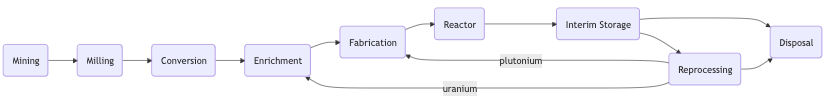
\includegraphics[scale=0.55]{images/nfc/closed_fc.png}
      \caption{Hypothetical Closed Fuel Cycle}
      \label{fig:closed_fc}
\end{figure}

% How do international treaties and agreements affect nuclear fuel cycle activities?
% In the emerging stage of the \gls{nfc}


% What opportunities exist for innovation and improvement in the nuclear fuel cycle?

\subsection{Front End of the Fuel Cycle}
\label{sec:front_end}
At the time of writing, the 2024 "Red Book" from the \gls{nea} and \gls{iaea}
has not been released, as such we will extrapolate trends from the 2022 joint
report on Uranium availability in the world. The 2022 "Red Book" report covers
January 2019 to January 2021 and updates the projections from 54 countries of
their uranium supply and resources through 2040 \cite{nea_red_book_2022}.

Globally, Australia continues to hold the largest resources (inferred and
reasonably assured) of uranium at roughly 28 \% of the world's total; however,
total identified recoverable resources declined 2\% from 2019 to 2021--in
contrast with slight increases reported in previous versions of the report--as
countries increased mining efforts, reclassified economic viability of inferred
resources, and currency values fluctuated with inflation. Among more
well-established uranium exporters like Australia, Kazakhstan re-evaluations of
inferred resources accounted for decreases in nearly every quality category,
while relatively newer exporters, Mongolia and Niger, reported increases in
inferred resources \cite{nea_red_book_2022}. This work focuses on the \gls{usa}
explicitly and does not incorporate geospatial information.

The \gls{usa} has been importing more uranium than it has been producing
domestically as shown in Figure \ref{fig:foregin_u3o8}. This trend is expected
to continue as the \gls{usa} has only recently begun to invest in new uranium
mines since the 1980s. The \gls{usa} has been importing uranium from countries
like Canada, Australia, and Kazakhstan, which have large uranium deposits.

\begin{figure}[!h]
   \centering
   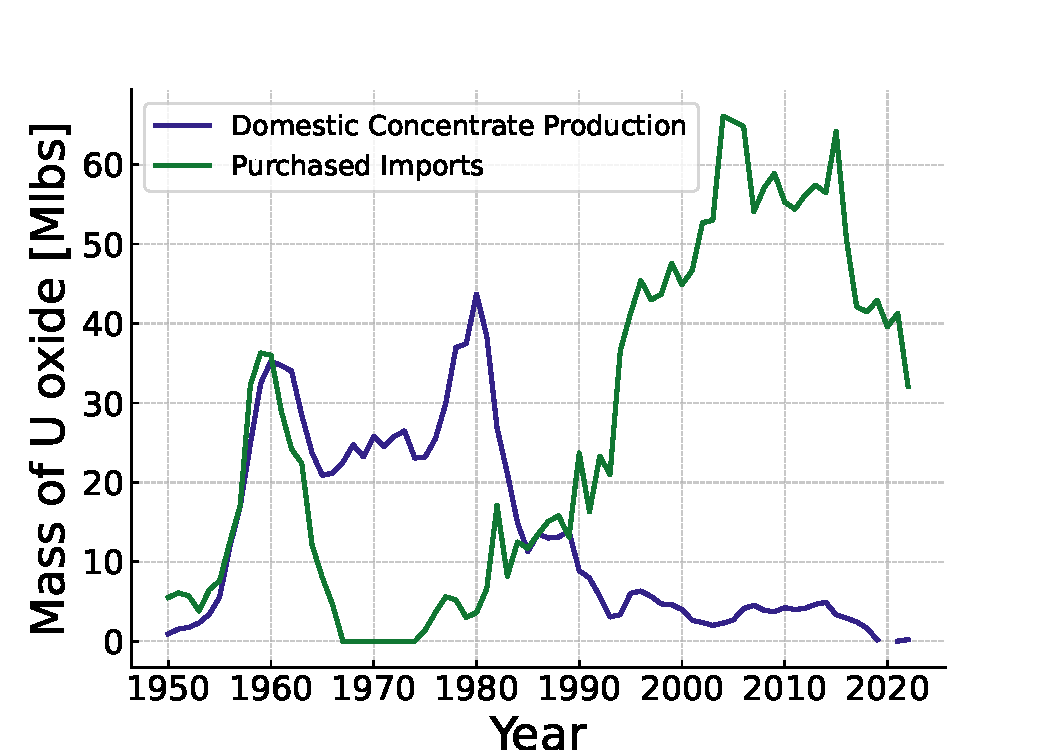
\includegraphics[scale=0.8]{images/intro/uranium_production_imports.pdf}
   \caption{Foreign and domestic uranium purchases over time \cite{eia_monthly_energy_review_2024}.}
   \label{fig:foregin_u3o8}
\end{figure}

As the 2022 "Red Book" notes, there is a growing body of literature surrounding
our understanding of best practices for environmental stewardship and
remediation of mines. Once common practices of strip, pit, and underground
mining are beginning to be replaced with more sustainable practices that
minimize the environmental impact of mining. One method that has garnered
interest in the uranium mining community is in-situ leaching, wherein workers
inject a leaching solution into the ground to dissolve the uranium and then
pump the solution to the surface for processing \cite{insitu_review_2024}. The
paradigm shift in uranium mining is from a focus on burial depth to a focus on
geological properties. In-situ leaching is limited to areas with favorable
permeabilities, but the reduced labor intensity, simplified infrastructure
requirements, and lower environmental impact make it an attractive option for
uranium mining where applicable.

In-situ leaching also reduces the extent of the milling process as the ratio of
desirable material to non-desirable material is higher in the leaching solution
than in the resultant material from traditional mining. The milling process
generally involves crushing the ore into a fine powder and then leaching the
uranium from the ore with a sulfuric acid solution. Workers then extract the
uranium from the solution and convert it into yellowcake, a concentrated form
of uranium oxide \cite{milling_uranium_2022}. The yellowcake is then shipped to
a conversion facility where it is converted into uranium hexafluoride, a gas
that cools to a liquid and then a solid before it is transported to be
enriched. Uranium hexafluoride is attractive in the enrichment process because
fluorine has only one naturally occurring isotope and is therefore easy to
ensure isolation from the uranium.

Up to the enrichment stage of the fuel cycle, we have described a process
almost entirely agnostic to the end use of the uranium fuel. Leaving the
conversion stage of the fuel cycle is a colorless, volatile, and radioactive
solid material. The goal of the enrichment process is to achieve a specific
concentration or weight percent of $^{235}$U with respect to the other uranium
isotopes. Today, the enrichment process is typically done using centrifuges,
which separate the isotopes based on their mass; however, we historically used
gaseous diffusion, and could potentially use laser enrichment if it becomes
economically viable. In this work we do not distinguish between enrichment
services, instead making use of \gls{swu}, which we will expand on in Section
\ref{sec:swu}.

The enriched uranium is then converted into uranium dioxide, which is
fabricated into fuel. For our fleet of large \glspl{lwr}, the fuel is made into
pellets, which are stacked into rods, and collected into assemblies. This is
not the case for every reactor design, as some reactors make use of prismatic
fuel elements, pebble fuel elements, or liquid fuel elements. As with
enrichment, the fabrication stage of the fuel cycle is simplified in this work
and we do not incorporate explicit details of the fabrication process.

\subsection{Reactor Operation}
\label{sec:reactor_operation}
Up to now, everything we have laid out is part of the front end of the fuel
cycle. The part of the \gls{nfc} where the fuel is used in the reactor is
neither at the front nor back of the fuel cycle. As such, we have created a
separate section for it, despite the comparatively small amount of processes we
outline here. Inside the reactor core, the fuel generates heat through fission,
which produces steam, thereby driving a turbine to generate electricity. The
fuel remains in the reactor for several years, depending on the design of the
reactor and the enrichment of the fuel. This interstitial phase of the
\gls{nfc} is now complete.


\subsection{Back-End of the Fuel Cycle}
\label{sec:back_end}
% used fuel storage
After the fuel has been in the reactor for several years, it is removed and
stored in a spent fuel pool. After cooling, the fuel is moved to dry cask
storage, where it will remain until a long-term solution is implemented. As
this work does not focus on closed-fuel cycles, we do not consider the
reprocessing of the fuel in this description of the \gls{nfc}.

% How is radioactive waste managed and disposed of?
When it comes to considerations for a long-term repository for the used fuel,
we must consider the macroscopic and microscopic effects of the environment on
the repository. On a macroscopic level, climate change will drive shorelines to
move, permafrost to recede, and congenital ice sheets to melt. Translating
these well-known effects into chemical consequences that dictate the design of
a repository will require site-specific adaptations on several fronts. Special
attention must be given to the impact in the first few thousand years, as this
period will exhibit the highest activity. In the case of meltwater exposure,
water saturated with dissolved $O_2$ could infiltrate some repositories,
potentially altering the oxidizing conditions \cite{gurban_hydrochemical_2001}.
Consequently, regulators considering the 100,000-year perspective of a
potential repository must account for proximity to such meltwater sources to
meet the demands imposed by a changing climate.

It is additionally possible that sites experiencing reducing conditions will
continue to do so. However, another consideration is how the salinity of
groundwater will be influenced by the changing climate. Changes in salinity
affect density, which could either exacerbate or mitigate the spread of
contaminants in the event of exposure outside the repository
\cite{gurban_hydrochemical_2001}. This change in salinity also has the
potential to interact differently with canisters, necessitating that proactive
regulators ensure containment is designed to withstand a changing environment
over the repository's lifetime.

An additional layer of microscopic consideration for these regulatory concerns
is the imminent deployment of new nuclear fuels with different compositions and
forms. Some fuels are designed with pyrolytic carbon matrices that can
immobilize decay products for much longer than current fuel forms. As new fuel
technologies are deployed, it follows that \gls{nfc} facilities will adapt
accordingly. These changes, although seemingly slight (the fuel will likely
still be uranium-based), can have significant consequences over 100,000 years
of storage \cite{hyland_post_closure_2013}.